\chapter{Realisation of a demonstrator}
\textbf{keep it small and simple} 
%Outline of the technologies used to fabricate and assemble your structures, if applicable. Detailed processes belong in the appendix. If numerous types of structures were fabricated, or assembly technology is extensive, there may be more than one of these chapters. \textbf{Characterization} Description of the means developed and employed to characterize the devices or systems that have been fabricated.
%The realisation of the demonstrated concepts on a hybrid substrate was one goal of this thesis, to show its feasibility.
The demonstrator consists of several multi assembled \gls{ab:mmic} with a filter network built by discrete \gls{ab:smd} decoupling capacitors.
Therefore the realised demonstrator is a hybrid test circuit.
To avoid building a too complex structure the resolution of the \gls{ab:dac} was restricted to two bit.
With two bit resolution there are already four inputs which need to be controlled.
This four input have to be controlled via a high speed digital signal with a peak to peak value of 5 volt, to ensure that the input \gls{ab:hemt} is fully opened or fully closed.
The input control signal is amplified due to a pre amplifier for the frequency from kHz to several tens of GHz.
This broadband is needed for the harmonics of the rectangular signal.
Then the bias voltage is set due to a bias tee.
This makes the setup more complex. 
If a third bit was added this control setup would increase, too.

Therefore a two layer substrate could be used to keep it small and simple.
For the realisation two different versions of the demonstrator were designed. 
Both realisations were based on the former work from Stephan Maroldt who designed the chips. 
\section{Demonstrator using DDRi\_X6 and DDRi\_Y6 chips}
\begin{enumerate}
	\item Highside driver load transistor voltage connected to Vdd
	\item Highside driver load transistor voltage connected to Vout
\end{enumerate}
A pad ,which is surrounded by the conductive layer with its via holes, is used because the chips DDrixy6 are connected to its metallized backside by through hole vias. In order to realize a Vdd supply voltage at the drain of this power mosfet and the output signal at the source, the chip does not be soldered onto the gnd layer of the substrate. 
Because otherwise the circuit would not work in a proper form.
The schematic show that the output power transistor stage has to switch in a push-pull format. So the drain of the highside transistor is connected to Vdd which is realized with the chips on the rf pad. The lowside transistor and its driver circuit is the chip soldered on the substrate.
\section{Demonstrator using DDRi\_2C chips}
\begin{enumerate}
	\item Highside driver load transistor voltage connected to Vdd
	\item Highside driver load transistor voltage connected to Vout
\end{enumerate}
In fact of that for this chips no backside connection to the chip backside exists, this chip can be directly soldered onto the substrate without losing the functionality.
In contrast to the other version, here the gnd pads of the chip have to be bonded onto the substrate gnd. This version could be more convenient due to the better heat dissipation.
The used chips:
\begin{enumerate}
	\item DDRi\_X6 and DDRi\_Y6
	\item DDRi\_2C
\end{enumerate}
were designed but unfortunately they do not have a simulation model which would make it easier to simulate the outcome. \\
The design and processing of a MMIC structure containing the Riemann Pump circuit was beyond the scope of this thesis.
% so it was a nice way to proof the concept to use the former designed chips.
In addition to this MMIC chips some discrete components were used, e.g.bypass capacitors to filter out undesired distortion frequencies which could lead to oscillation which makes the circuit potentially instable/unstable.\\
In the realisation and layout progress many things must be considered.\\
The circuit is build on a hybrid assembly which combines the MMIC with the discrete SMD components on a Rogers 4003 substrate.\\
The input and output lines on the substrate were \gls{ab:msl} which were tuned to \SI{50}{\ohm}.
Tuned in this sense means, the lines were created with the right width, length and depth on the correct substrate with a special thickness.
Important for the design of the input lines were that these lines are of same length due to phase angle issues for switching at the same time. 
The output line also was tuned to 50 ohm to guarantee a proper measurement with standard rf cables.\\
Also it would tried to get a proper distance between the lines to avoid any coupling. \\
An important thing was that the bond wires of in- and output lines to the \gls{ab:mmic} chips should be of the same length. The idea is that the high frequency digital signal are not allowed to have phase angles, because the switches have to switch all at the same time. Timing problems are expected to occur within the measurement. \\
In addition to this, the chips are producing power which produce a lot of heat and this heat has to dissipate.
One important point is the heat dissipation. The chips have to dissipate the heat away form them. 
Here the different layouts comes into play.
In a first version the chips (DDRi\_XY6) are mounted on an island/pad and in the near of that a conducting layer with via holes are set to spread the heat over the air bridge (ambient temperature) to the via hole to the backside. 
This is not the optimal way to dissipate the heat, but the only to handle some heat dissipation.
In a second version the other chips (DDRi\_2C) which were not connected through via holes to the metallized backside of the chip, are soldered on the conducting substrate of the rogers hybrid substrate. This conductive layer have a lot of via holes to the cooled backside of the rogers substrate. 
The heat could spread directly from the backside of the chip which is metallized through the via holes of the substrate to the substrates backside.
This second version could be the more efficient/convenient way.
But the chips designed by S. Maroldt are a little bit older and therefore the taping of the wafer could be not as good as the newer ones. - what are other reason to not use this one?\\
 Due to this heat dissipation problem it would resign to package the chips into an QFN package\\
For bonding, the normal 25u Au bonds are used. The bonds length are given to the assembly limits for spacing of conducting layers of the manufacturer.\\
In- and output connectors are SMA jack connectors, to connect to standard RF cables.\\ 
A few bypass capacitors are used based on the experience and experimental advice of some colleagues, rule of thumb. 
Suitable capacitors were those with a high \gls{ab:esr} which means a bad q-factor, and of course the temperature range, the voltage range should be suitable to the purpose(flatten mag of imp vs. freq broadband good).
(Bypassing and operating frequency not necessarily linked to each other. Bypassing a greater range than the potential operating frequency) (Culture Cargo principle). The first bypass capacitance the chip supply voltage sees is a MMIC cap directly assembled near to the supply pin of the chip.\\
Maybe the number of via holes on the substrate to the backside could create some additional inductance. keep that in mind for the measurement.\\
The dc supply slowly increase due to the fact of thermal issues. 
The Vss is -5V and Vdd is 15V\\
Capacitive coupling could be a problem, through the dc supply lines to the input lines.
What about the coupling from the substrate backside to the conducting layer of the substrate? 
What about inductive coupling via the via holes or so??
Other coupling?\\
The chips are different in order that the DDRi\_2C chip is not connected via through hole via to the metallized backside of the chip. 
Therefore this chip can be soldered to the substrate, which has a lot of via holes for thermal dissipation, without loss of functionality.

	\begin{itemize}
		\item chip with gnd vias on island and nearby copper plate with thermal vias to cool down the ambient temp of the MMIC
		\item chip without gnd via, direct soldered on the copper with thermal vias
	\end{itemize}

The two layouts were ordered at Contag in Berlin on 22nd Feb.
The components needed to be ordered are ordered at digikey in the Netherlands.

\begin{figure}[htb!]
	\centering
  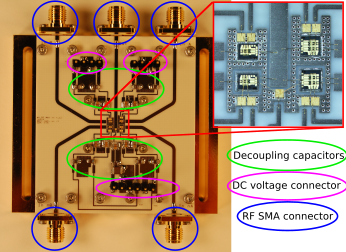
\includegraphics{Demonstrator_edited_newScale.pdf}
	\caption{Assembled demonstrator}
	\label{fig:assembledDemonstrator}
\end{figure}

\textit{temperature dissipation critical. heat transfer versus electric conduction for the high side chips.}
 %An order were made with Axel Tessmann and M. Zink, Riessle to get the chips from the manufactured wafer in 2011.